% Chapter 3
\chapter{Envelopes and keyboard} % Main chapter title
\label{Chapter3} % For referencing the chapter elsewhere, use \ref{Chapter1} 
\lhead{Chapter 3. \emph{Envelopes}} % This is for the header on each page - perhaps a shortened title
\textsf{\textsl{Written by Kenneth Piot}}
%----------------------------------------------------------------------------------------
\section{Envelopes}
\subsection{General meaning of the envelope}
When the synthesizer generates a sound, then the frequency of that signal determines how the signal sounds. The frequency, however, does not affect the loudness of the sound. Loudness is determined by the amplitude. At the start, when a sound gets generated or at the end, when the sound dies out, the amplitude changes. The way the amplitude changes during the life cycle of the sound is the envelope.\\
Figure \ref{fig:envA} gives an example of the envelope of a signal. It is divided into 3 sections. The first section is called "attack". It is the rise of the amplitude at the start of the signal generation. The amplitude is at its maximum at the end of the attack. The time the total attack takes is predetermined but if the generation of the signal gets disrupted before the attack time is expired, then the envelope goes directly to the last(third) section, called "release".\\
The release is the section where the signal dies out. The amplitude will decrease until it finally becomes 0. The release time is just like the attack time predetermined.\\
The second section is called "decay". In this section of the envelope the signal's amplitude decreases from the final amplitude of the attack to a lower one. The decay time is also predetermined.\\
\begin{figure}[!ht]
  \hfill
  \begin{minipage}[t]{.45\textwidth}
    \begin{center}  
      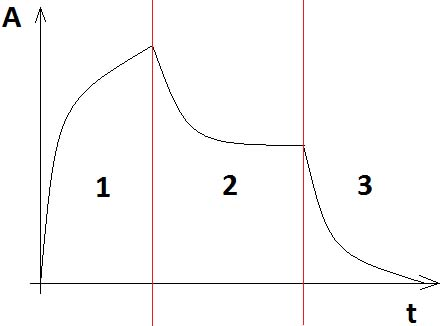
\epsfig{file=envA, scale=0.40}
      \caption{Example of envelope}
      \label{fig:envA}
    \end{center}
  \end{minipage}
  \hfill
  \begin{minipage}[t]{.45\textwidth}
    \begin{center}  
      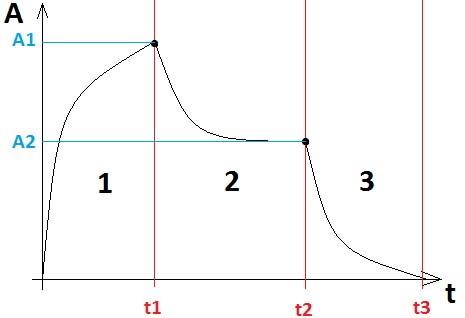
\epsfig{file=envB, scale=0.40}
      \caption{Envelope with the parameters for the equations}
      \label{fig:envB}
    \end{center}
  \end{minipage}
  \hfill
\end{figure}\\
There is also a fourth section but it is not shown in figure \ref{fig:envA}. This section is called "sustain". It is actually the section between the decay and the release. The reason it is not shown is because sustain time is not predetermined. The sustain lasts until, in the case of a synthesizer , a button is released after the attack and decay. Then the envelope passes into the release. The amplitude of the sustain is constant and is equal to the final amplitude of the decay.
%----------------------------------------------------------------------------------------
\subsection{Mathematical equations}
The attack, decay and release all have a different but similar equation, respectively equations \ref{eq:1}, \ref{eq:2} and \ref{eq:3}:
\begin{equation}
A = \frac{A_{1}}{t_{1}^{slope_{1}}} \cdot t^{slope_{1}}
\label{eq:1}
\end{equation}
\begin{equation}
A = \frac{A_{2} - A_{1}}{ (t_{2} - t_{1})^{slope_{2}}} \cdot (t  -t_{1})^{slope_{2}} + A_{1}
\label{eq:2}
\end{equation}
\begin{equation}
A = \frac{- A_{2}}{(t_{3} - t_{2})^{slope_{3}}} \cdot (t - t_{2})^{slope_{3}} + A_{2}
\label{eq:3}
\end{equation}
The variables A1, A2, t1, t2 and t3 are represented in figure \ref{fig:envB}. Slope 1, slope2 and slope 3 are the slopes of section 1, 2 and 3 respectively. \\
Figure \ref{fig:slopes} shows examples of the attack with different slopes. The straight line in the middle is an attack with a slope of 1. If slope becomes larger than 1, the attack will rise first at a slow rate and then faster in an exponential way. The larger the slope, the faster the attack will rise at the end. If the slope is larger than 0 but smaller than 1, the attack will first rise fast and then slower in an exponential way.
\begin{figure}[htbp]
\centering
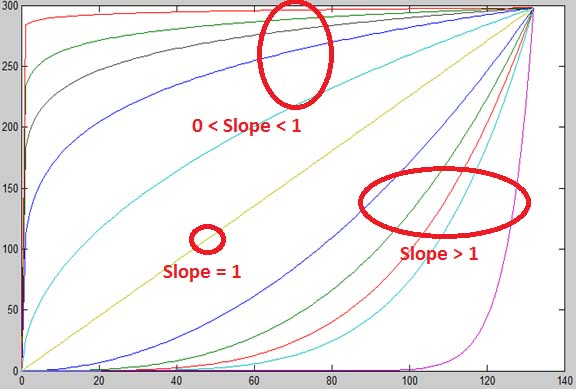
\includegraphics[height=6cm]{envC}
\rule{30em}{0.5pt}
\caption{Different slopes for the attack}
\label{fig:slopes}
\end{figure}
%----------------------------------------------------------------------------------------
\subsection{Envelopes and modulation}
When modulating a signal, only the carrier is hearable (Bjorn does not agree with this!). With an envelope you can make a sound for example fade in or out. The modulators only change the original (carrier) signal but the modulators aren't directly hearable.\\  
The modulators, however, do have an envelope as well. We know that when we modulate a signal, the modulation is also dependent on the modulation index ''I". This value is an indication for how hard the original signal gets modulated. The envelope of the modulators change the value ''I". In this way a modulation is affected by the envelope.
%----------------------------------------------------------------------------------------
\subsection{Envelopes in the program}
Each operator has a variable" envEn"(Bool), "time"(int) and "count"(int). The parameter envEn is a boolean and it is used to switch the envelopes on or off. While modulating (Bjorn: also without modulation), the program checks if envEn is true. If this is the case time increases by 1. If this is not the case time and count each become 0. If envEn is true and time is equal to the sampling frequency (96000Hz), count increases by one. This is to indicate that a period of 1 second has elapsed. \\
Below is the algorithm for the envelopes shown. The variable "totTime" is the total time of the envelope. The program checks if the envelopes are enabled. If this is true, it checks if the totTime
 $<=$ endPointATKt, $>$ endPointATKt and $<=$ endPointDECt or $>$ endPointRELt. This is a way for the program to know in which phase of the envelope totTime is located (attack, decay or release). If totTime is greater than endPointRELt, the variable envEn becomes false so the envelope will repeat itself as long as the user doesn't turn off the envelopes.
If the envelopes are not enabled, the amplitude of the wave is constant and equal to the amplitude the user chose on the interface. 
\begin{alltt}
for(i=0; i<4; i++)
{
   (op[i].envEn == TRUE) ? (op[i].env.time)++ : (op[i].env.time = op[i].env.count = 0);
   if(op[i].envEn == TRUE && !(op[i].env.time%=sampleFreq)) op[i].env.count++;
}

if(op->envEn)
{
   totTime = op->env.time + op->env.count * sampleFreq;	

   if(totTime <= endPointATKt)
      result=(op->amplitude/(powf(endPointATKt,slope1)))*powf(totTime,slope1);
   else if(totTime > endPointATKt && totTime <= endPointDECt)
      result=((((endPointDECa - op->amplitude)/powf((endPointDECt - endPointATKt),slope2)) 
             *powf((totTime - endPointATKt),slope2)) + op->amplitude);
   else if(totTime > endPointDECt && totTime <= endPointRELt)
      result=(((-endPointDECa/powf((endPointRELt-endPointDECt),slope3))*powf((totTime 
             - endPointDECt),slope3)) + endPointDECa);
   else if(totTime > endPointRELt)
      op->envEn = FALSE;			
}
else  result = op->amplitude;

return result;
\end{alltt}
%----------------------------------------------------------------------------------------
\subsection{Problems that occurred during the course of the project}
There were a lot of problems with the envelopes. At first there was only one variable time for all the operators. This way the envelopes worked too but it was confusing to program with and the envelope would not start from the beginning. It was also not possible to make the envelopes repeat properly without individual timers for each operator (Bjorn: not true!). \\
Another problem was the variable count. At first count would not increase of each operator individually. The counts of all enabled envelopes would increase at the same time when time\%=96000 would equal to 0. The problem that would occur was that count would only increase every 4 seconds instead of 1. Every time a block of 1024 samples is processed, time increases by 1024. This, however, would cause time\%=96000 to be only 0 when time reached 384000 which is equal to 96000*4.\\
To solve this problem we would let the counts of the enabled envelopes increase in the function "createSignal" itself. The function \verb+updateEnvelopes()+ increases the counts of all enabled envelopes. Now count would increase properly every second. Another problem occurred when modulating. If we for example modulate with 2 operators. If time would become 96000, count of operator 1 and operator 2 would both increase. If the envelope of the first operator would then be calculated there would be no problem. The problem would occur with the second operator. Count of this operator would have increased at the same time as count of the first operator. This would cause the envelope of the second operator to skip samples because totTime of that envelope would not have the right value. This problem could be solved by making the counts of the enabled envelopes increase individually. 
\begin{alltt}
void createSignal(Operator *op, int t)
{
   int i;
   float scalar;
   scalar=powf(2.0,23.0);
   switch(op->wave)
   {	
   case SINE:
      for(i=0; i<NUM_SAMPLES; i++)
      {
            op->signal[i] = envelope(op, &t)*sin( 2.0 * 3.141592 * 
                                            op->frequency / sampleFreq * t );
            t+= 1;
            if(!(t\%=sampleFreq)) updateEnvelopes(); //nrT++
            t\%=sampleFreq;
      }
      break;
	}
}
\end{alltt}
\begin{remark}
Please see the section ''Key functions'' \ref{code:createSignal} for the correct version of this function and without unused variables and double operations.
\end{remark}
%----------------------------------------------------------------------------------------
\section{Keyboard control}
The synthesizer must be able to play different music notes with the press of a key on the keyboard like a piano.\\ 
Figure \ref{fig:piano} shows the labview algorithm for keyboard control of the synthesizer. This sample algorithm checks if "B" on the keyboard is pressed. In short these are the steps the program goes through to accomplish this: 
\begin{enumerate}
\item The algorithm first checks if the Boolean to switch on the keyboard is true. If this is the case, the algorithm goes to step 2 (this step is not shown on figure \ref{fig:piano1}).
\item The pressed key gets registered by the program. On figure \ref{fig:piano1} the keyboard is shown with all the buttons.
\item The name of the pressed key is stored in an array and the pressed keys on the keyboard interface get a darker color as long as the keys are pressed. Labview assumes you are using a QWERTY keyboard so in figure 2 the requirement is "Z" but on an AZERTY keyboard this is "W". The user doesn't have to know this because he/she only has to look at the interface of the keyboard.
\item The case structure checks if the name of the key is equal to "Z" in this case.
\item If the key is pressed: The associated key on the interface becomes darker and the frequency of the sound that gets created becomes 31Hz in this case. The frequencies of the other buttons are $2^{\frac{1}{12}}$ times the frequency of the previous one. For example, the frequency of "S" is $2^{\frac{1}{12}}$ times the frequency of "W" and the frequency of "X" is $2^{\frac{1}{12}}$ times the frequency of "S".
If no key is pressed: frequency of the sound automatically becomes 0.
\item The while loop repeats.
\end{enumerate}
We made 2 octaves of buttons for the interface which means that every button in the second octave has a frequency that is twice the frequency of the corresponding button on the first octave.
\begin{figure}[htbp]
\centering
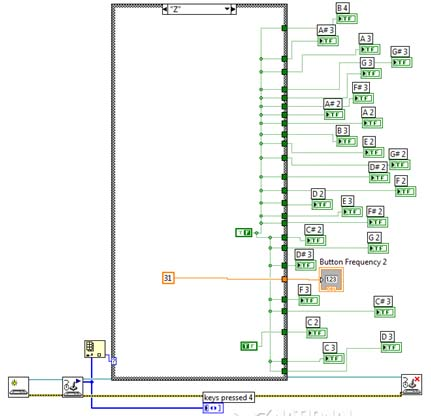
\includegraphics[height=10cm]{piano}
\rule{30em}{0.5pt}
\caption{Labview algorithm for keyboard control}
\label{fig:piano}
\end{figure} \\
\begin{figure}[htbp]
\centering
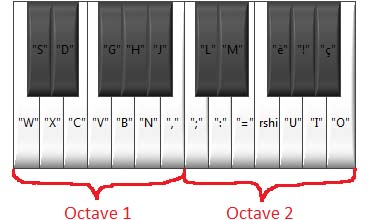
\includegraphics[height=5cm]{piano1}
\rule{30em}{0.5pt}
\caption{Keyboard buttons}
\label{fig:piano1}
\end{figure} 
